\section{System Architecture} \label{sec:system-architecutre}
\todo[inline]{explain the statistics collection unit and the scheduler (in more detail)}
\todo[inline]{update the figure (system architecture)}
Our proposed deployment platform comprises four components; pipeline manager, data manager, scheduler, and an independent SGD run-time. 
Figure \ref{fig:system-architecture} gives an overview of the architecture of our system and the interactions among its components.
%The data manager first stores the incoming training observations in a buffer and then passes them on to the model manager.
%The model manager incrementally updates the model using the training observations.
%The model manager is also responsible for receiving prediction requests.
%Once it receives a request, it uses the latest version of the model to make a prediction and returns the result to the user.
%Both the scheduler and the data manager components are constantly communicating with each other and with the model manager, to obtain the latest statistics, such as the model quality and buffer size.
%This in turn helps us to tune the scheduling and sampling rate for future iterations of SGD. 
%Next, we explain each component of the system in more detail.


\begin{figure}[t]
\centering
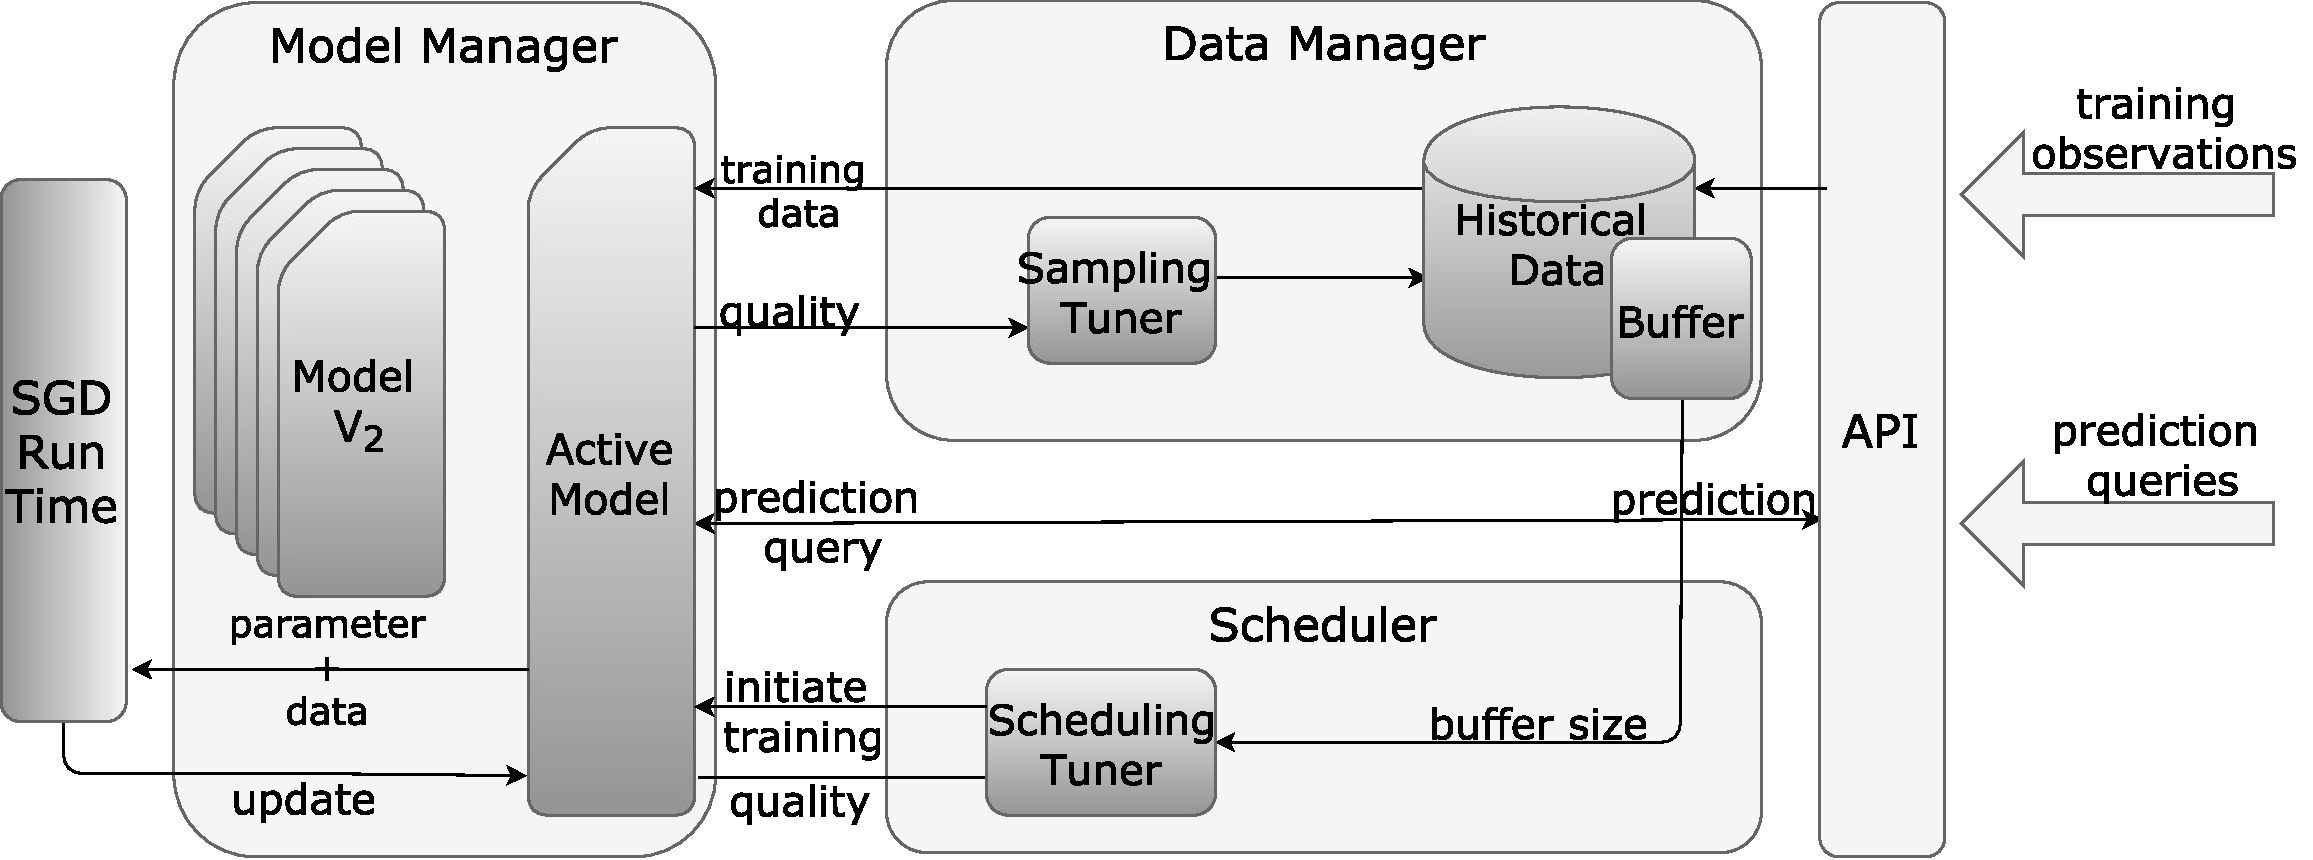
\includegraphics[width=\columnwidth]{../images/system-architecture-final.pdf}
\caption{System Architecture}
\label{fig:system-architecture}
\end{figure}


\subsection{Scheduler}\label{scheduler}
The scheduler component is responsible for scheduling new iterations of SGD.
Intuitively, the best time to execute an iteration is when the system is not under heavy load.
A new iteration of SGD is also executed when the system receives more training data than can be handled by the intermediate buffer.
If the model is not updated with the new training items frequently, the quality decreases.
This decrease in the quality is more rapid if the distribution of the data is changing.
In our prototype, the scheduling rate is controlled by a user defined parameter, \textit{max\_buffer\_size}.
When the intermediate buffer's size reaches \textit{max\_buffer\_size}, the scheduler executes a new iteration of SGD.
It is important to note that the scheduling rate affects the quality of the model.
In Section \ref{evaluation}, we investigate the effect of scheduling rate on model quality.
If no new training data is available, the model parameters will eventually converge and any further training iterations will not have any effect on the model quality.
\todo[inline]{R3: How is the convergence detected?}
Therefore, the scheduler component has to communicate with the model manager in order to detect whether the model parameters have converged and stop further iterations until more training data becomes available.

\subsection{Data Manager} \label{data-manager}
The data manager component is responsible for storage of historical data, processing the incoming training data, and providing the SGD run-time with new batch of training data for every iteration.

Historical data is typically large and may not fit in the memory or disk of a single machine. 
The data manager handles the communication with the underlying storage unit.
When new training data becomes available, the data manager append the incoming data to the existing historical data.
Moreover, the incoming training data are forwarded to the pipeline manager to update the statistics required by the pipeline components.

When a new iteration of SGD is scheduled to run, the data manager is responsible for providing the batch of training data.
The data manager can provide the next batch of training data in two different mode, namely, \textit{sample-then-append} or \textit{append-then-sample}.
In sample-then-append mode, the new training data that has arrived at the system is stored in an intermediate buffer in the memory.
The historical data is sampled and the resulting data is then combined the with data in the buffer.
The data manager makes the combined data available for the SGD run-time to execute the next iteration of SGD.
In append-then-sample mode, the new training data is appended to the historical data upon arrival.
The data manager then samples the historical data (that consists of the new training data) and provides the resulting dataset for the SGD run-time.

The two operation modes of data manager affects the way the deployed model is evolving over time.
In sample-then-append mode, every iteration of SGD uses the new training data in its entirely.
Therefore, there is a more emphasis on the recent data than the historical data.
While this is the more desirable method, it may lead to unstable updates, as the distribution of the data may change due to concept drift or anomalies.
Append-then-sample mode assigns the same weight to every data point (new training and the historical data).
As a result, the update to the deployed model is more stable, however, the increase in model quality is smaller than sample-then-append mode.
In our experiments, we investigate the effect of the different operation mode on model quality and consumption.

%Different sampling strategies can be used to provide the sample.
%In our current prototype, the data manager uses a simple unified random sampling method to generate this sample.
%More advanced methods, such as Reservoir \cite{vitter1985random} or weighted random sampling can also be used to generate the sample.
%Reservoir sampling is typically used to generate samples from large datasets that do not fit in memory, whereas weighted random sampling is used when data elements have different weights.
%In an online machine learning scenario, recent items are more important for training the model and are assigned a bigger weight than older items.
%Therefore, weighted random sampling can generate samples that can contribute to the training of a better model.

Data manager also allows for new training datasets to be registered while the model is being served.
The new dataset is merged with the existing historical data and immediately becomes available for next iterations of SGD.

\subsection{Pipeline Manager} \label{pipeline-manager} 
\todo[inline]{discuss statistics collection and update the Listing to show apis for statistics gathering. Discuss what are default ones that being collected and how users can have custom statistics collected and use them inside or outside of the system.}
\todo[inline]{Mention how pipelines that are trained outside can be used in the system and how they can be exported again (current prototype uses spark serialized object and we (can) support  PMML}
An important part of the system is the model manager component.
It is responsible for storing the model, answering prediction queries, and performing incremental and batch updates to the model.
Listing \ref{pipeline-manager-api} shows the API of the model manager.
The API is used to interact with other components as well as end-users of the system.
The scheduler component uses \textit{update} and \textit{update\_iteration} to instruct the model manager to perform incremental or batch updates (one iteration of SGD) to the model.
Upon a new prediction query, the \textit{predict} method is called to provide the end-user with the label of the given input.

\noindent\begin{minipage}[t]{\linewidth}
\begin{lstlisting}[language=java, basicstyle=\small\ttfamily, frame=tb ,columns=fullflexible,
showstringspaces=false,label=pipeline-manager-api,caption=Model Manager API, numberstyle=\tiny]
def update(x,y)

def update_iteration(X,Y)

def predict(x): Label

def error_rate(X_test, Y_test): Double

\end{lstlisting}
\end{minipage}


The \textit{error\_rate} method returns the error rate of the model using the provided test dataset.
As described earlier, constant monitoring of the quality is required in order to adjust the scheduling and sampling rate.
When the error rate is stagnating, the model has converged using the existing data.
Therefore the model manager informs scheduler not to schedule any new iterations until new training observations have arrived at the system.
\todo[inline]{R3: How is this done exactly?}
Similarly as explained in Section \ref{data-manager}, an increase in the error rate may indicate a change in distribution of the data.
As a result, reducing the sampling rate will place more emphasis on recent data (in the intermediate buffer) and help adapt the model to the changes in the distribution.

The model manager also keeps track of the changes that are made to the model.
The model is updated both through incremental learning and SGD-iteration.
The model manager creates snapshots of the model in two different scenarios; after a series of incremental updates are made and after each training iteration.
\todo[inline]{R3: What is the algorithm here?}
This versioning of the models is essential.
When there is a rapid change in the distribution of the incoming data (a sudden concept drift) or when there are anomalies in the data, it is sometimes necessary to revert back to a version before the change in distribution occurred.
In case of concept drift, new training iterations should be scheduled that only use the data in the buffer.
Moreover, in case of anomalies in the data, they have to be identified and discarded before any further model updates could happen.

\subsection{SGD Run-Time} 
All components of our model serving system described so far are not limited to any specific run-time.
We have decoupled the components from the actual run time of the system.
Any system capable of performing incremental and batch SGD updates efficiently are suitable options for our system.
Apache Flink \cite{carbone2015apache} and Apache Spark \cite{zaharia2010spark} are distributed data processing platforms that work with data in memory and have support for iterative algorithms, which makes both of them ideal options for our SGD run-time.
In our current prototype, we are using Apache Spark \cite{zaharia2010spark} as our SGD run-time.

The model manager is the component responsible for communicating with the SGD run-time.
In the current version of our prototype, the model manager requests Spark to perform both incremental and batch updates to the model.
Both types of updates are supported by the built in machine learning library of Spark.
The choice of run-time for SGD slightly influences the data manager as well.
In our prototype, historical data is stored on the Hadoop Distributed File System (HDFS) \cite{shvachko2010hadoop}.

\todo[inline]{R3: The paper has a point that not only the resource consumption is reduced by incremental update, but also the prediction accuracy can be improved due to adapting the model to newly seen data. The system uses a sampling component to use a subset of historical data in each SGD update. However, a non-incremental retraining can also achieve the same adaptation by weighing towards the newly seen data (e.g., learning with concept drifting). Therefore, the ideas of incremental update and adaptation to concept drift should not be confused. The evaluation in this paper does not clearly decouple them. BD: Interesting insight. We have to address this.}